% Compile with XeLaTeX!!!
\usepackage{ifxetex}
\ifxetex
\pdfpagewidth=3\paperwidth
\pdfpageheight=\paperheight
\usepackage{fontspec}
\defaultfontfeatures{Mapping=tex-text}
\input{UBScala/fontspec}
\setmainfont{UBScala}
\setsansfont{UBScalaSans}
\else
\fi

\usepackage[dvipsnames,usenames]{xcolor}
%%UNIBA-Colors
\definecolor{unibablueI}{HTML}{00457D}
\definecolor{unibablueII}{HTML}{336A97}
\definecolor{unibablueIII}{HTML}{6690B1}
\definecolor{unibablueIV}{HTML}{99B5CB}
\definecolor{unibablueV}{HTML}{CCDAE5}

\definecolor{unibayellowI}{HTML}{FFD300}
\definecolor{unibayellowII}{HTML}{FFDC33}
\definecolor{unibayellowIII}{HTML}{FFE566}
\definecolor{unibayellowIV}{HTML}{FFED99}
\definecolor{unibayellowV}{HTML}{FFF6CC}

\definecolor{unibagreenI}{HTML}{97BF0D}
\definecolor{unibagreenII}{HTML}{ACCC3D}
\definecolor{unibagreenIII}{HTML}{C1D86E}
\definecolor{unibagreenIV}{HTML}{D5E59E}
\definecolor{unibagreenV}{HTML}{EAF2CF}
%Not CD, darker versions
\definecolor{nounibagreenI}{HTML}{82A50B}
\definecolor{nounibagreenII}{HTML}{708C0A}

\definecolor{unibaredI}{HTML}{E6444F}
\definecolor{unibaredII}{HTML}{EB6972}
\definecolor{unibaredIII}{HTML}{F08F95}
\definecolor{unibaredIV}{HTML}{F5B4B8}
\definecolor{unibaredV}{HTML}{FADADC}
%Not CD, darker versions
\definecolor{nounibaredI}{HTML}{CC3D47}
\definecolor{nounibaredII}{HTML}{B3363E}

\definecolor{unibagrayI}{HTML}{878783}
\definecolor{unibagrayII}{HTML}{9F9F9C}
\definecolor{unibagrayIII}{HTML}{B7B7B5}
\definecolor{unibagrayIV}{HTML}{CFCFCE}
\definecolor{unibagrayV}{HTML}{E7E7E6}

%%%%%%%%%%%%%%%%%%%%%%%%%%%%%%%%%%%%%%%%%%%%%%%%%%%%%%%%%%%
% TIKZ Configuration
%%%%%%%%%%%%%%%%%%%%%%%%%%%%%%%%%%%%%%%%%%%%%%%%%%%%%%%%%%%
\usepackage{tikz}
\usetikzlibrary{positioning,patterns,calc}


\renewcommand*\foldmarkrule{.3mm}
\renewcommand*\foldmarklength{5mm}

\usepackage{amsmath}
%\usepackage[T1]{fontenc}
\usepackage{textcomp}
\usepackage{mathptmx}
%\usepackage[scaled=0.9]{helvet}
\makeatletter
\def\ptmTeX{T\kern-.1667em\lower.5ex\hbox{E}\kern-.075emX\@}
\DeclareRobustCommand{\ptmLaTeX}{L\kern-.3em
        {\setbox0\hbox{T}%
         %\vb@xt@ % :-)
         \vbox to\ht0{\hbox{%
                            \csname S@\f@size\endcsname
                            \fontsize\sf@size\z@
                            \math@fontsfalse\selectfont
                            A}%
                      \vss}%
        }%
        \kern-.12em
        \ptmTeX}
\makeatother
%\let\TeX=\ptmTeX
%\let\LaTeX=\ptmLaTeX
\usepackage{shortvrb}
%\MakeShortVerb{\|}
\usepackage{url}
\usepackage{graphicx}
\usepackage{longtable}
\usepackage{colortbl}
\usepackage{multirow,varwidth,array}
\definecolor{LIGHTGRAY}{gray}{.9}

%%%%\renewcommand{\descfont}{\normalfont}
\newcommand\Lpack[1]{\textsf{#1}}
\newcommand\Lclass[1]{\textsf{#1}}
\newcommand\Lopt[1]{\texttt{#1}}
\newcommand\Lprog[1]{\textit{#1}}

\newcommand*\defaultmarker{\textsuperscript\textasteriskcentered}

%\usepackage[colorlinks=true, urlcolor=unibablueI]{hyperref}

\makeatletter
\def\maketitle{%
\null
  \thispagestyle{empty}%
  \vfill
%  \begin{center}
%  
% 
% \begin{tikzpicture}[yscale=-0.1, xscale=0.1, node distance=3mm,outer sep = 0pt, inner sep=0pt]
%\tikzset{grid/.style={gray,very thin,opacity=1}}
%\tikzstyle{default}=[anchor=north west]
%\tikzstyle{bg}=[fill=unibayellowV, opacity=.75, anchor=north west]    
%
%\draw[bg, rounded corners] (0,0) rectangle (10*\textwidth,21);
%%\draw[grid] (0,0) grid (10*\textwidth,3*\textheight);
%\node[default] (gi) at (2,2) {
%        
\includegraphics[width=.2\textwidth]{images/gi.png}
%    };
%\node[default] (itg) [right=of gi] {
%        
\includegraphics[width=.25\textwidth]{images/itg.png}
%    };
%\node[default] (dft) [right=of itg] {
%        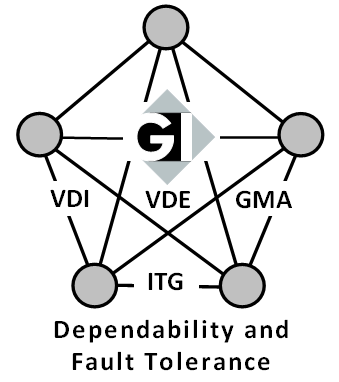
\includegraphics[width=.2\textwidth]{images/dft.png}
%    };
%\node[default] (mmb) [right=of dft] {
%        
\includegraphics[width=.2\textwidth]{images/mmb.png}
%    };
%\end{tikzpicture} 
% \end{center}
 \vspace{4ex}
 \begin{minipage}{.05\textwidth}
 \hfill
 \end{minipage}
 \begin{minipage}{.9\textwidth}
  \begin{center}
    {\Huge\sf \textcolor{unibablueI}{\@title}\par}%
    \vskip .5ex
    {\Large\sf \textcolor{unibablueI}{\@author}\par}%
    \vskip .5ex
    {\Large\sf \textcolor{unibablueI}{\@date}\par}%
  \end{center}%
  \hfill
   \end{minipage}
  %\vfill
  \null
  }
\makeatother

\renewcommand\familydefault{\sfdefault}

\usepackage{rotating} 